\documentclass[a4paper,margin,line]{resume}
\usepackage[defblank]{paralist}
\usepackage{pdfpages}
\usepackage{blfootnote}
\usepackage{anysize}
\usepackage[pdftex, unicode]{hyperref}
\hypersetup{
	pdftitle={Russell Harmon's Resume},
	pdfauthor={Russell Harmon},
	pdfborder={0 0 0},
	% Not sure if this is needed.
	unicode=true
}
\marginsize{0.375in}{1.875in}{0.5in}{0.5in}
\setdefaultitem{\footnotesize \textbullet}{}{}{}{}{}
\setdefaultleftmargin{0em}{}{}{}{}{}
\setdefaultenum{(a)}{(1)}{}{}{}{}
\newcommand{\rurl}[1]{\hfill {\footnotesize \url{#1}}}
\newcommand{\rdate}[1]{\hfill {\small #1}}
\renewcommand{\employer}[5]{\item[#1] - #2 \rdate{#3} \\* #4 \rurl{#5} \\*}
\begin{document}
\name{\Large Russell E. Harmon}
\begin{resume}
\section{\mysidestyle Contact \\ Information} \vspace{2mm}
	\begin{asparablank}
		\item Rochester Institute of Technology \hfill 2710 Avenue J NW
		\item 39 Nathaniel Rochester Hall \hfill Winter Haven, FL 33881
		\item Rochester, NY 14623 \hfill \href{mailto:russ@eatnumber1.com}{russ@eatnumber1.com}
		\item (863) 514-7014 \hfill
		\href{http://blog.eatnumber1.com/}{blog.eatnumber1.com}
	\end{asparablank}

\section{\mysidestyle Education}
	\begin{compactdesc}
		\item[Rochester Institute of Technology] - Rochester, NY \rdate{September 2006 - Present}
		\begin{compactitem} { \small
			\item Major: B.S./M.S. Computer Science
			\item Minor: Music
			\item Expected graduation: June 2012
		} \end{compactitem}
	\end{compactdesc}

\section{\mysidestyle Experience}
	\begin{asparadesc}
		\employer{SafeNet Inc}{Belcamp, MD}{June 2008 - Present}{Engineering
		Intern}{http://www.safenet-inc.com/}

		\small
		Worked on the SafeNet Management Console (SMC) on a team of seven. SMC is
		a web application built on Java, JBoss, Hibernate and JSF which manages high
		speed network encryption devices that SafeNet manufactures, including
		top-secret devices. While working at SafeNet, my responsibilities included
		\begin{inparaenum} \item creating requirements documents, \item implementing
		requirements, \item testing and \item fixing defects. \end{inparaenum} Some
		of the specific tasks that were assigned while working there included
		implementing IPv6 support and implementing support for multiple SMC servers
		managing the same device (distributed devices).
		\normalsize
		\\
		\employer{New York City Department of Education}{Bronx, NY}{September 2002 -
		June 2006}{IT Specialist}{http://schools.nyc.gov/}

		\small
		Worked at Lehman High School while I was a student there. The work there
		included \begin{inparaenum} \item setup and maintain the computer systems,
		\item repair and maintain the network, \item diagnose and eliminate viruses
		and malware on the school's network and computer systems and \item audit the
		network for malicious activity. \end{inparaenum}
		\normalsize
		\\
		\employer{New York Sailing \& Yacht Club}{Bronx, NY}{June 2001 - August 2005}{Launch
		Operator}{http://www.startsailing.com/}
		
		\small
		Worked at the New York Sailing \& Yacht Club as the launch operator. The
		work involved taxiing patrons to their boats moored in the harbor. While
		there, I also received a boating license in small craft operation.
		\normalsize
	\end{asparadesc}

\section{\mysidestyle Technical Skills \& Certifications}
	\begin{compactdesc}
		\item[Languages] \begin{inparaenum} { \small
			\item Java
			\item C/C++
			\item BASH/SH \& other KSH derived shell scripting languages
			\item Python
		} \end{inparaenum}
		\item[Operating Systems] \begin{inparaenum} { \small
			\item Linux -
			\begin{inparablank}
				\item Gentoo,
				\item Debian based,
				\item OpenWRT
			\end{inparablank}
			\item Solaris
			\item Windows
			\item OSX
		} \end{inparaenum}
		\item[Hardware] \begin{inparaenum} { \small
			\item Server Maintenance
			\item Networking
			\item Network Security
		} \end{inparaenum}
		\item[Tools] \begin{inparaenum} { \small
			\item \LaTeX
			\item Microsoft Office
			\item Vim
			\item Idea
		} \end{inparaenum}
		\item[Certifications] \begin{inparaenum} { \small
			\item Cisco Academy, with honors (terms 1 and 2)
			\item A+
			\item MOUS (Word)
		} \end{inparaenum}
	\end{compactdesc}

\section{\mysidestyle Extracurricular}
	\begin{asparablank}
		\item US FIRST Robotics Team 1230 - {\small Lead programmer} \rurl{http://www.usfirst.org/}
		\item CSH - {\small Computer Science House} \rurl{http://www.csh.rit.edu/}
		\item Rocking the Boat - {\small Built a boat for children from the South
		Bronx} \rurl{http://www.rockingtheboat.org/}
		\item City Island Computer Services - {\small Age 10}
	\end{asparablank}

\section{\mysidestyle Honors \& Awards}
	\begin{asparablank}
		\item NYC Regional Robotics Award winner - {\small 27th place nationally}
		\item Visual Basic programming award for academic excellence 2005
		\item First Place Sailing Award 2000, 2002
	\end{asparablank}

\section{\mysidestyle Special Accomplishments}
	\begin{asparablank}
		\item At age 8, built my first computer. At age 12, attended my first
		programming class at Lehman College.
		\item Designed and implemented an encryption algorithm using a
		combination of transposition and substitution.
	\end{asparablank}

\section{\mysidestyle Personal \\ Strengths}
	I am a person who loves to tinker. I spend the majority of my free time
	working on personal projects. As a result, I've found that I have become very
	good at picking up new ideas quickly, and expanding what I already know with
	little more than the internet and a direction.

\end{resume}
\pagebreak[4] % The 4 makes it a VERY INSISTENT requirement for a page break.
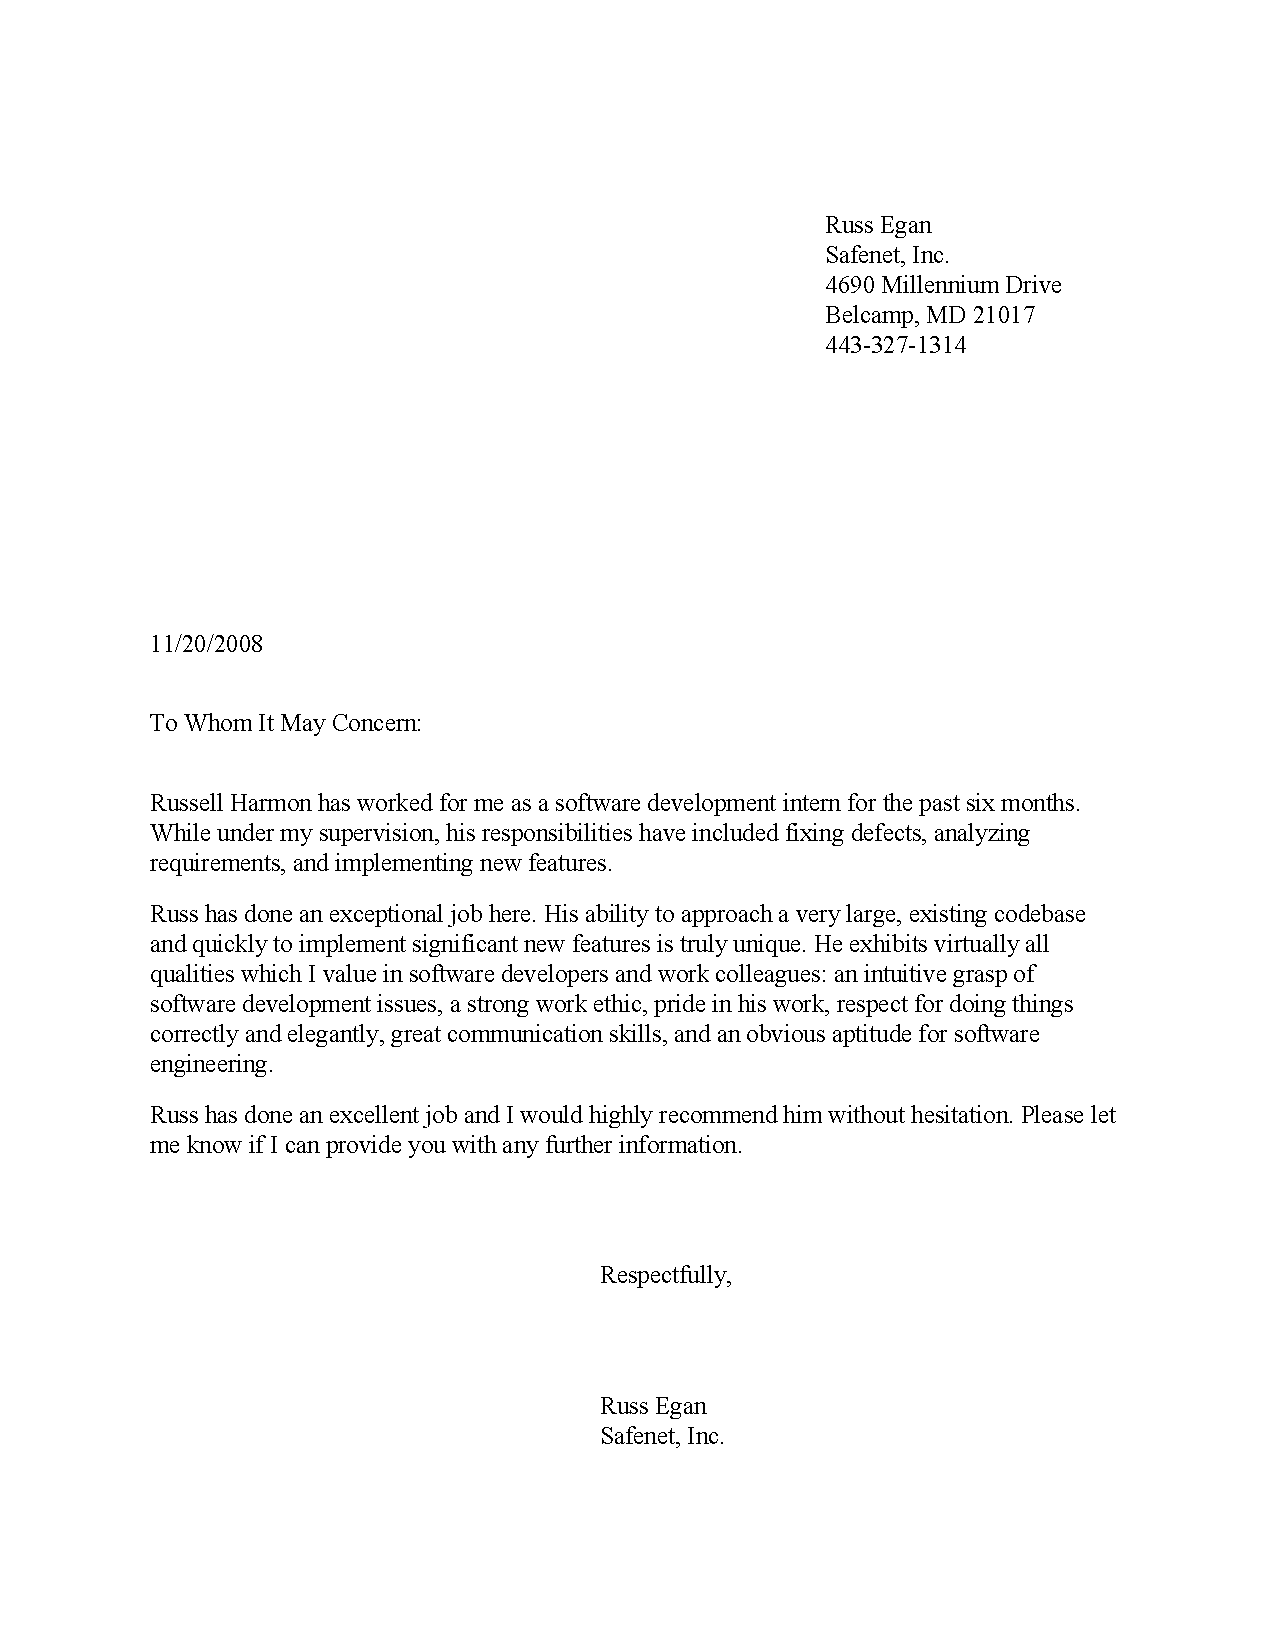
\includepdf[offset=-94 0,pages=1]{sfnt-recommendation}
\end{document}
